% !TEX root = ../Preparazione alle olimpiadi.tex

\chapter{Pattern Algoritmici}

In questo capitolo verranno introdotti alcuni pattern algoritmici classici utilizzati nella risoluzione efficiente dei problemi computazionali.  
Queste tecniche rappresentano strategie ricorrenti nella progettazione degli algoritmi e consentono di ridurre la complessità computazionale, migliorando le prestazioni rispetto a soluzioni brute force.

In particolare, verranno analizzati i seguenti pattern:
\begin{itemize}
	\item \textbf{Sliding Window}, una strategia basata su finestre mobili per l'elaborazione di sottoarray o sottostringhe contigue;
	\item \textbf{Bitmask}, una rappresentazione compatta degli insiemi che consente di gestire combinazioni e stati in modo efficiente tramite operazioni sui bit.
	\item \textbf{Prefix Sum}, una tecnica di preprocessing che permette di rispondere rapidamente a interrogazioni su intervalli;
\end{itemize}

Lo studio di questi pattern fornisce una base fondamentale per affrontare problemi di programmazione competitiva e per comprendere concetti più avanzati della progettazione algoritmica.





\section{Sliding Window}

La tecnica della \textit{Sliding Window} (finestra mobile) è una strategia algoritmica utilizzata per analizzare sottoarray o sottostringhe contigue di una sequenza di dati in modo efficiente.  
Essa si basa sul mantenimento di una finestra che scorre progressivamente lungo la struttura dati, evitando ricalcoli ridondanti e consentendo di ridurre la complessità computazionale rispetto a soluzioni di tipo brute force.

L’idea principale consiste nel definire due indici che delimitano l’inizio e la fine della finestra e nell’aggiornare dinamicamente le informazioni associate alla finestra corrente (come somme, conteggi o massimi) man mano che la finestra viene spostata.

A seconda del problema, la dimensione della finestra può essere:
\begin{itemize}
	\item \textit{fissa}, quando la finestra ha lunghezza costante;
	\item \textit{variabile}, quando la finestra si espande o si contrae in base a determinate condizioni.
\end{itemize}

Grazie a questo approccio, molti problemi che richiederebbero un tempo di esecuzione quadratico $O(n^2)$ possono essere risolti in tempo lineare $O(n)$.  
La tecnica della Sliding Window è ampiamente utilizzata in ambiti quali l’elaborazione di array, stringhe e flussi di dati, e rappresenta uno strumento fondamentale nella progettazione di algoritmi efficienti.

\newpage
\noindent \textbf{Sliding Window fissa} 
\medskip

Supponiamo di avere un \texttt{vector} $A = (A_0, A_1, \dots, A_{N-1})$ e di voler determinare la somma massima degli elementi appartenenti a sottoarray contigui di lunghezza fissa $k$.

Un approccio ingenuo consiste nel calcolare la somma di tutti i possibili sottoarray di lunghezza $k$, ottenendo una complessità computazionale pari a $O(N \cdot k)$.  
Tale soluzione risulta inefficiente per valori elevati di $N$ e $k$.

Il codice di questo approccio brute force è il seguente:

\begin{lstlisting}
	#include <bits/stdc++.h>
	using namespace std;
	
	int main() {
		int N, k;
		cin >> N >> k;
		
		vector<int> A(N);
		for (int i = 0; i < N; i++) {
			cin >> A[i];
		}
		
		int maxSum = INT_MIN;
		
		// ciclo su tutte le finestre
		for (int i = 0; i <= N - k; i++) {
			int currentSum = 0;
			
			// calcolo la somma della finestra [i, i+k-1]
			for (int j = i; j < i + k; j++) {
				currentSum += A[j];
			}
			
			maxSum = max(maxSum, currentSum);
		}
		
		cout << maxSum << endl;
		
		return 0;
	}
	
\end{lstlisting}

La tecnica della \textit{Sliding Window} consente di risolvere il problema in tempo lineare $O(N)$ mantenendo una finestra di dimensione costante $k$ che scorre lungo il vettore.  
Inizialmente si calcola la somma dei primi $k$ elementi. Successivamente, la finestra viene spostata di una posizione verso destra sottraendo l’elemento che esce dalla finestra e aggiungendo l’elemento che entra (figura \ref{fig:pattern-algoritmici:sliding-window}).





Indicando con $[left, right]$ gli estremi della finestra, con $right - left + 1 = k$, l’aggiornamento della somma può essere espresso come:
\[
S_{\text{nuovo}} = S_{\text{precedente}} - A_{left} + A_{right+1}
\]

Dove con $A_{left}$ intendiamo l'elemento che esce dalla finestra dopo il suo scorrimento, $A_{right+1}$ intendiamo l'elemento che entra nella finestra.

Ripetendo tale procedura fino a raggiungere la fine del vettore, è possibile determinare la somma massima tra tutte le finestre considerate. 

\begin{figure}[H]
	\centering
	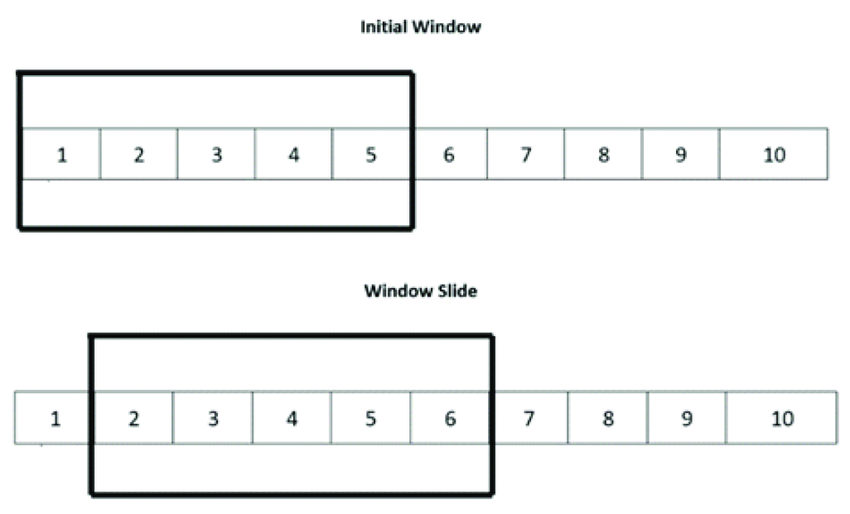
\includegraphics[width=0.6\textwidth]{immagini/4 - Pattern Algoritmici/Sliding window.png}
	\caption{Sliding Window fissa con $k = 5$. In questo caso, per ogni aumento del margine destro ($right$) vi è anche un aumento del margine sinistro ($left$)}
	\label{fig:pattern-algoritmici:sliding-window}
\end{figure} 

La codifica con la Sliding Window fissa è la seguente:

\begin{lstlisting}
#include <bits/stdc++.h>
using namespace std;

int main() {
	int N, k;
	cin >> N >> k;
	
	vector<int> A(N);
	for (int i = 0; i < N; i++)
	cin >> A[i];
	
	int maxSum = INT_MIN;
	int windowSum = 0;
	int left = 0;
	
	for (int right = 0; right < N; right++) {
		windowSum += A[right];  // aggiungo l'elemento entrante
		
		// se la finestra supera k elementi, rimuovo quello uscente
		if (right - left + 1 > k) {
			windowSum -= A[left];
			left++;
		}
		
		// aggiorno il massimo
		if (right - left + 1 == k)
		maxSum = max(maxSum, windowSum);
	}
	
	cout << maxSum << endl;
	
	return 0;
}

\end{lstlisting}

Questo approccio evita il ricalcolo completo della somma per ogni sottoarray e permette di ridurre la complessità temporale da $O(N \cdot k)$ a $O(N)$.

\vspace{0.5cm}

\noindent \textbf{Sliding Window variabile} 

\medskip

Supponiamo di avere un \texttt{vector} $A = (A_0, A_1, \dots, A_{N-1})$ e di voler determinare la massima somma di un sottoarray contiguo tale che la somma non superi un certo valore $M$ (oppure soddisfi un'altra condizione definita dal problema).  

In questo caso, la lunghezza della finestra non è più fissa, ma varia dinamicamente durante lo scorrimento.  

Ancora una volta, l'approccio ingenuo consiste nel verificare tutte le possibili finestre, ottenendo una complessità pari a $O(N^2)$, che risulta inefficiente per valori elevati di $N$.

Il codice brute force è analogo al caso precedente, ma con due cicli annidati su tutti i possibili intervalli.

\medskip

La tecnica della \textit{Sliding Window variabile} consente di risolvere il problema in tempo lineare $O(N)$ mantenendo una finestra definita dagli indici $[left, right]$.  
Si procede nel seguente modo:

\begin{itemize}
	\item L'indice $right$ scorre l'intero array aggiungendo gli elementi alla somma della finestra.
	\item Quando la somma o la condizione della finestra non è più soddisfatta, si sposta $left$ verso destra rimuovendo gli elementi usciti dalla finestra.
	\item Ad ogni passo si aggiorna il valore massimo o la quantità desiderata.
\end{itemize}


La codifica in C++ è la seguente:

\begin{lstlisting}
#include <bits/stdc++.h>
using namespace std;

int main() {
	int N, M;
	cin >> N >> M;  // N elementi e somma massima consentita
	
	vector<int> A(N);
	for (int i = 0; i < N; i++){
		cin >> A[i];
	}
	
	
	int maxSum = 0;
	int windowSum = 0;
	int left = 0;
	
	for (int right = 0; right < N; right++) {
		windowSum += A[right];  // aggiungo l'elemento entrante
		
		// riduco la finestra finche' la condizione non è soddisfatta
		while (windowSum > M && left <= right) {
			windowSum -= A[left];
			left++;
		}
		
		// aggiorno il massimo
		maxSum = max(maxSum, windowSum);
	}
	
	cout << maxSum << endl;
	
	return 0;
}
\end{lstlisting}

In questo caso:

\begin{enumerate}
	\item $right$ espande la finestra includendo nuovi elementi. 
	\item $left$ contrae la finestra quando la condizione non è più rispettata. 
	\item  $maxSum$ viene aggiornato solo quando la finestra soddisfa la condizione. 
	\item Complessità: $O(N)$, perché ogni elemento entra ed esce dalla finestra al massimo una volta.
\end{enumerate}

La figura \ref{fig:pattern-algoritmici:sliding-window-mobile} illustra il meccanismo di espansione e contrazione della sliding window.


\begin{figure}[H]
	\centering
	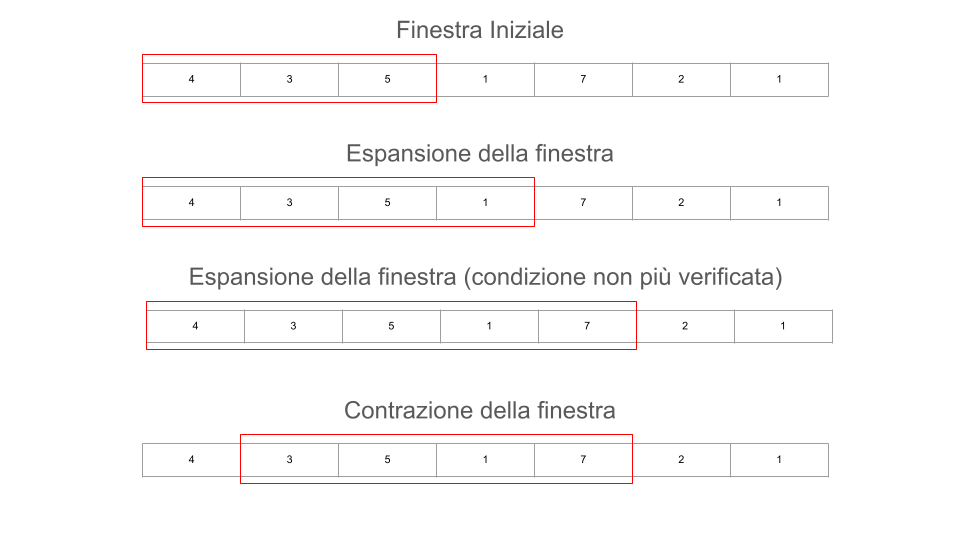
\includegraphics[width=1\textwidth]{immagini/4 - Pattern Algoritmici/Sliding window mobile.png}
	\caption{Sliding Window variabile. I margini $left$ e $right$ sono indipendenti e vengono gestiti in maniera che la finestra rispetti una certa condizione}
	\label{fig:pattern-algoritmici:sliding-window-mobile}
\end{figure} 





Questo schema è molto utilizzato per problemi con vincoli dinamici sulla finestra, come:
\begin{itemize}
	\item somma massima/minima sotto un certo limite,
	\item conteggio massimo di elementi con una proprietà,
	\item lunghezza massima di sottosequenze valide, ecc.
\end{itemize}




\section{Bitmask}
La tecnica del \textit{bitmask} è un metodo che consente di rappresentare sottoinsiemi di un insieme finito utilizzando la rappresentazione binaria degli interi.  
Ogni bit di un numero intero viene associato a un elemento dell’insieme: il valore $1$ indica la presenza dell’elemento nel sottoinsieme, mentre il valore $0$ ne indica l’assenza.

Dato un insieme di $n$ elementi $\{e_0, e_1, \dots, e_{n-1}\}$, ogni sottoinsieme può essere rappresentato tramite un intero compreso tra $0$ e $2^n - 1$.  
Incrementando progressivamente di una unità tale valore (da $0$ fino a $2^n - 1$) e osservandone la rappresentazione binaria, si ottengono tutte le possibili combinazioni di presenza e assenza degli elementi, ovvero tutti i sottoinsiemi dell’insieme dato.

La tecnica del bitmask può essere vista come una forma di bruteforce sui sottoinsiemi; tuttavia, grazie alla rappresentazione compatta degli stati e all’uso delle operazioni bitwise, consente un’implementazione più efficiente e leggibile rispetto a un approccio ingenuo.

Essa è particolarmente utile nei problemi di programmazione competitiva e di progettazione di algoritmi in cui è necessario:
\begin{itemize}
	\item generare tutti i sottoinsiemi di un insieme;
	\item verificare rapidamente l’appartenenza di un elemento a un insieme;
	\item ridurre l’uso della memoria rispetto a strutture dati più complesse.
\end{itemize}




















\section{Prefix Sum}

La tecnica delle \textit{Prefix Sum} (somme prefisse) è un metodo di preprocessing che consente di calcolare in modo efficiente la somma degli elementi di un array su un determinato intervallo.  
L’idea fondamentale consiste nel costruire un nuovo array in cui ogni elemento rappresenta la somma cumulativa degli elementi precedenti.

\vspace{0.5cm}

Supponiamo di avere un array di $N$ interi del tipo

\begin{equation*}
	a_0, a_1, ... , a_n
\end{equation*}

e di voler rispondere alla domanda: qual è la somma degli elementi da $a_l$ ad $a_r$? Con $0 \le l \le r < N$.
In altre parole ci stiamo chiedendo qual è la somma dall'elemento $l$ all'elemento $r$.

Per risolvere questo problema potremmo essere tentati di utilizzare una tecnica del tipo \textbf{brute force} che, in C++, potremmo codificare così:

\begin{lstlisting}[language=C++]
	#include <bits/stdc++.h>
	using namespace std;
	
	int main(){
		int N;
		cin >> N;
		
		vector<int> v(N); // vettore di dimensione N
		
		for(int i = 0; i < N; i++){
			cin >> v[i];
		}
		
		int l, r;
		cin >> l >> r; // si assume 0 <= l <= r < N
		
		int somma = 0;
		
		// brute force: somma degli elementi nell'intervallo [l, r]
		for(int i = l; i <= r; i++){
			somma += v[i];
		}
		
		cout << somma << endl;
	}
\end{lstlisting}

Supponiamo di dover calcolare $Q$ somme su intervalli $[l, r]$, 
differenti per ogni query $Q_i$. Qual è la complessità computazionale totale in questo caso?

Proviamo a scrivere il codice seguendo, ancora una volta, un approccio \textbf{brute force}.

\begin{lstlisting}[language=C++]
	#include <bits/stdc++.h>
	using namespace std;
	
	int main(){
		int N;
		cin >> N;
		
		vector<int> v(N); // vettore di dimensione N
		for(int i = 0; i < N; i++){
			cin >> v[i];
		}
		
		int Q;
		cin >> Q; // numero di query
		
		for(int q = 0; q < Q; q++){
			int l, r;
			cin >> l >> r; // si assume 0 <= l <= r < N
			
			int somma = 0;
			for(int i = l; i <= r; i++){
				somma += v[i]; // brute force: somma degli elementi nell'intervallo [l, r]
			}
			
			cout << somma << endl;
		}
		
		return 0;
	}
\end{lstlisting}
\bigskip
\noindent \textbf{Costo Computazionale}: \\

Il costo computazionale dell'approccio brute force è il seguente:
\begin{itemize}
	\item $O(Q)$ per il ciclo esterno sulle $Q$ query
	\item $O(N)$ per il ciclo interno che calcola la somma nell'intervallo $[l, r]$ nel caso peggiore
\end{itemize}

Pertanto, la complessità computazionale totale è:

\begin{equation*}
	O(Q) \cdot O(N) = O(Q \cdot N)
\end{equation*}

Questo approccio, sebbene semplice e intuitivo, non è ottimale per valori grandi di $N$ e $Q$. 

\medskip
\noindent La soluzione più efficiente utilizza la tecnica delle \textbf{somme prefisse} (prefix sum).  
L'idea consiste nel creare un secondo vettore $S$ di dimensione $N$ in cui ogni elemento contiene la somma cumulativa degli elementi dell'array originale $v$ fino a quella posizione:

\begin{equation*}
	S[i] = v[0] + v[1] + \dots + v[i] \quad \text{per } i = 0, 1, \dots, N-1
\end{equation*}

In questo modo, la somma di un intervallo qualsiasi $[l, r]$ può essere calcolata in tempo costante tramite:

\begin{equation*}
	\sum_{i=l}^{r} v[i] =
	\begin{cases}
		S[r], & \text{se } l = 0 \\
		S[r] - S[l-1], & \text{se } l > 0
	\end{cases}
\end{equation*}

In altre parole, una volta costruito il vettore $S$ (con complessità $O(N)$), per calcolare una qualsiasi somma da $l$ ad $r$ non faccio altro che eseguire il seguente calcolo:

\begin{equation}
	S[r] - S[l-1]
\end{equation}

Quindi, ad esempio, per calcolare la somma degli elementi dall'indice 3 all'indice 6, basta prendere la somma cumulativa di tutti gli elementi fino all'indice 6 e sottrarre la somma cumulativa fino all'indice 2. In questo modo si ottiene direttamente la somma degli elementi dall'elemento 3 all'elemento 6, estremi inclusi.

Come detto, il preprocessing per costruire l'array delle somme prefisse richiede $O(N)$, mentre ogni query può essere risolta in $O(1)$.  
Pertanto, la complessità totale diventa:

\begin{equation*}
	O(N) + O(Q) = O(N + Q)
\end{equation*}

Questa soluzione è estremamente più efficiente rispetto al brute force quando sia $N$ che $Q$ sono grandi.

Proviamo a codificare il problema:

\begin{lstlisting}[language=C++]
	#include <bits/stdc++.h>
	using namespace std;
	
	int main(){
		int N;
		cin >> N;
		
		vector<int> v(N); // vettore di dimensione N
		for(int i = 0; i < N; i++){
			cin >> v[i];
		}
		
		vector<int> prefix(N); // vettore delle somme prefisse
		prefix[0] = v[0];      // il primo elemento è lo stesso di v[0]
		
		// costruisco le somme prefisse
		for(int i = 1; i < N; i++){
			prefix[i] = v[i] + prefix[i-1]; // sommo l'elemento corrente v[i] con la somma precedente
		}
		
		// Una volta costruito prefix, la somma di un intervallo [l, r] si calcola in O(1)
		int Q;
		cin >> Q;
		
		for(int q = 0; q < Q; q++){ 
			int l, r;
			cin >> l >> r;
			
			int somma;
			if(l == 0)
			somma = prefix[r]; // se l = 0, la somma e' prefix[r]
			else
			somma = prefix[r] - prefix[l-1]; // altrimenti sottraggo prefix[l-1]
			
			cout << somma << endl;
		}
		
		return 0;
	}
\end{lstlisting}

\bigskip
\noindent \textbf{Costo Computazionale}: \\

Il costo computazionale è il seguente:
\begin{itemize}
	\item $O(N)$ per riempire il vettore $prefix$ (riga 17)
	\item $O(Q)$ per il ciclo esterno sulle $Q$ query
	\item $O(1)$ per il calcolo di $somma$
\end{itemize}

Pertanto, la complessità computazionale totale è:

\begin{equation*}
	O(N) + O(Q) = O(N + Q)
\end{equation*}

Rispetto all'approccio \emph{brute force} (come mostrato in precedenza), 
questo metodo permette un notevole risparmio di tempo quando $Q$ ed $N$ sono molto grandi.



\subsection{C - Index × A(Continuous ver.)}
\label{problema:prefix:C-IndexxA}

\href{https://atcoder.jp/contests/abc267/tasks/abc267_c}{Link al problema}
\noindent Time limit = 1.00s, Memory limit = 512 MB
\bigskip

\subsubsection*{Problem Statement}

You are given an integer sequence $A = (A_1, A_2, \dots, A_N)$ of length $N$.
Find the maximum value of $\sum_{i=1}^{M} i \times B_i.$ for a contiguous subarray $B = (B_1, B_2, \dots, B_M)$ of $A$ of length $M$.

\subsubsection*{Notes}
A contiguous subarray of a number sequence is a sequence that is obtained by removing 
$0$ or more initial terms and $0$ or more final terms from the original number sequence.

For example, $(2,3)$ and $(1,2,3)$ are contiguous subarrays of $(1,2,3,4)$, but $(1,3)$ and $(3,2,1)$ are not contiguous subarrays of $(1,2,3,4)$.

\subsubsection*{Constraints}
\begin{itemize}
	\item	$1 &\le M \le N \le 2\cdot10^5 \hspace{0.1cm}000$ 
	\item	$−2\cdot10^5 &\le A_i \le 2\cdot10^5\hspace{0.1cm}000\hspace{0.1cm}000$ 
	\item	All values in input are integer.
\end{itemize}

\subsubsection*{Input}

Input is given from Standard Input in the following format:

$N\ M$  

$A_1\ A_2\ \dots\ A_N$

\subsubsection*{Output}
Print the answer.

\subsubsection*{Sample Input1}
\begin{verbatim}
	4 2
	5 4 -1 8
\end{verbatim}

\subsubsection*{Sample Output1}
\begin{verbatim}
	15
\end{verbatim}


\vspace{0.5cm}

When $B=(A_3,A_4)$, we have $\sum_{i=1}^{M} i\cdot B_i=1\cdot(-1)+2\cdot8=15$. Since it is impossible to achieve 
16 or a larger value, the solution is 
15.

Note that you are not allowed to choose, for instance, 
$B=(A_1, A_4)$.

\subsubsection*{Sample Input2}

\begin{verbatim}
	10 4
	-3 1 -4 1 -5 0 -2 6 -5 3
\end{verbatim}

\subsubsection*{Sample Output2}
\begin{verbatim}
	31
\end{verbatim}


\bigskip
\noindent \textbf{Idea 1:} 

Il problema richiede di calcolare la seguente somma:

\begin{equation}
	S = \sum_{i=1}^{M} i \cdot B_i
\end{equation}

in modo tale che \(S\) sia massima, dove
\(B = (B_1, B_2, \dots, B_M)\) è un \textbf{sotto-array contiguo} della sequenza \(A\).

Un approccio intuitivo consiste nei seguenti passi:

\begin{enumerate}
	\item Consideriamo una \textbf{finestra di lunghezza \(M\)} che scorre lungo l'array \(A\).  
	Denotiamo questa finestra come \(B\) inizialmente posizionata sugli indici \(0, \dots, M-1\).
	
	\item Per la finestra corrente, calcoliamo la sommatoria richiesta:
	\begin{equation}
		S = \sum_{i=1}^{M} i \cdot B_i
	\end{equation}
	
	\item Spostiamo la finestra di \textbf{un passo verso destra} (cioè agli indici \(1, \dots, M\)) e ricalcoliamo la sommatoria \(S\).  
	Ad ogni passo, confrontiamo il valore corrente con il massimo trovato finora e aggiorniamo il massimo se necessario.
	
	\item Ripetiamo questo procedimento per tutte le finestre contigue di lunghezza \(M\) presenti in \(A\).
\end{enumerate}

Alla fine, il \textbf{massimo valore} ottenuto tra tutte le finestre corrisponde alla soluzione del problema.

Come possiamo calcolare la sommatoria richiesta?  
Ricalcolarla da zero per ogni finestra sarebbe molto dispendioso in termini computazionali (lasciamo al lettore l'implementazione di questo metodo).  
Perciò, dobbiamo trovare una strategia più efficiente.

Possiamo osservare che:

\begin{equation}
	\label{prefix:Cindex:equation:S}
	S = \sum_{i=1}^{M} i \cdot B_i = \sum_{j = left}^{right} (j - left + 1) \cdot A[j]
\end{equation}

dove con \(left\) indichiamo l'indice del limite sinistro della finestra e con \(right\) l'indice del limite destro.

Espandendo i termini della sommatoria, si può notare che la quantità all'ultimo membro della equazione \ref{prefix:Cindex:equation:S} è proprio $S$.

Infatti, considerando che $j$ parta da $left$ e finisca a $right = left+M-1$, $S$ diventa:


\begin{align}
	S &= \sum_{j = left}^{right} (j - left + 1) \cdot A[j] \\
	&= (left - left + 1) \cdot A[left] 
	+ (left + 1 - left + 1) \cdot A[left+1] + \notag \\
	&\quad + (left + 2 - left + 1) \cdot A[left+2] 
	+ \dots \notag \\
	&\quad + (left + M - 1 - left + 1) \cdot A[left + M - 1] \notag
\end{align}

Ovvero, in forma compatta:

\begin{equation}
	S = 1 \cdot A[left] + 2 \cdot A[left+1] + \dots + M \cdot A[right]
\end{equation}

Che è esattamente la quantità che vogliamo massimizzare.

\vspace{0.5cm}

Ripartendo quindi dalla equazione \ref{prefix:Cindex:equation:S}, possiamo riarrangiarla in questo modo

\begin{align}
	S &= \sum_{j = left}^{right} (j - left + 1) \cdot A[j] = \notag \\
	&= \sum_{j = left}^{right} j \cdot A[j] + (left - 1) \cdot \sum_{j = left}^{right} A[j]
\end{align}

Da qui possiamo notare due contributi importanti:
\begin{itemize}
	\item $\sum_{j = left}^{right} A[j]$ (contributo destro)
	\item $\sum_{j = left}^{right} j \cdot A[j]$ (contributo sinistro)
\end{itemize}

Creiamo quindi due vector prefix tali per cui l'i-esimo elemento è:
\begin{itemize}
	\item \(\text{prefix}[i] = A[0] + A[1] + \dots + A[i], \quad \text{per } i = 0, 1, \dots, N-1\)
	
	\item \(\text{w\_prefix}[i] = 0 \cdot A[0] + 1 \cdot A[1] + \dots + i \cdot A[i], \quad \text{per } i = 0, 1, \dots, N-1\)
\end{itemize}

Dopo aver costruito i due vettori, possiamo calcolare i due contributi in $O(1)$:

\medskip
\textbf{Contributo destro}

\[
\sum_{j = left}^{right} A[j] =
\begin{cases}
	\text{prefix}[right], & \text{se } left = 0,\\
	\text{prefix}[right] - \text{prefix}[left-1], & \text{se } left > 0
\end{cases}
\]

\textbf{Contributo sinistro}

\[
\sum_{j = left}^{right} j \cdot A[j] =
\begin{cases}
	\text{w\_prefix}[right], & \text{se } left = 0,\\
	\text{w\_prefix}[right] - \text{w\_prefix}[left-1], & \text{se } left > 0
\end{cases}
\]

\bigskip

\noindent	\textbf{Implementazione C++:}
\begin{lstlisting}[language=C++]	
	#include <bits/stdc++.h>
	using namespace std;
	
	int main()
	{
		int N, M;
		cin >> N >> M; // Leggiamo la lunghezza dell'array e la dimensione della finestra
		
		vector<int64_t> A(N);
		for (int i = 0; i < N; i++)
		{
			cin >> A[i]; // Leggiamo gli elementi dell'array
		}
		
		// COSTRUZIONE DEL VETTORE prefix
		// prefix[i] = somma dei primi i+1 elementi di A
		vector<int64_t> prefix(N);
		prefix[0] = A[0]; // il primo elemento della somma cumulativa è A[0]
		
		for (int i = 1; i < N; i++)
		{
			prefix[i] = A[i] + prefix[i - 1]; // somma cumulativa fino all'indice i
		}
		
		// COSTRUZIONE DEL VETTORE w_prefix
		// w_prefix[i] = somma pesata dei primi i+1 elementi: 0*A[0] + 1*A[1] + ... + i*A[i]
		vector<int64_t> w_prefix(N);
		w_prefix[0] = 0; // il primo elemento pesato è 0*A[0]
		
		for (int i = 1; i < N; i++)
		{
			w_prefix[i] = i * A[i] + w_prefix[i - 1]; // somma pesata cumulativa fino all'indice i
		}
		
		int left = 0;                 // limite sinistro della finestra
		int64_t ans = INT64_MIN;      // variabile per salvare il massimo valore trovato
		int64_t current_value;        // valore della sommatoria per la finestra corrente
		
		// Scorriamo l'array per calcolare tutte le finestre di lunghezza M
		for (int right = left + M - 1; right < N; right++)
		{
			// Assicuriamoci che la finestra sia lunga esattamente M
			while (right - left > M - 1)
			{
				left++; // spostiamo il limite sinistro verso destra
			}
			
			// CALCOLO DELLA SOMMA PESATA NELLA FINESTRA [left, right]
			if (left == 0)
			{
				// Se la finestra parte dall'inizio dell'array
				// allora la sommatoria pesata e' semplicemente w_prefix[right]
				// e aggiungiamo prefix[right] per correggere l'indicizzazione
				current_value = w_prefix[right] + prefix[right];
			}
			else
			{
				// Se la finestra parte da left > 0
				// Usiamo la formula generale per le somme pesate di una finestra
				current_value = (w_prefix[right] - w_prefix[left - 1])  
				- (left - 1) * (prefix[right] - prefix[left - 1]); 
			}
			
			// Aggiorniamo il massimo trovato
			ans = max(current_value, ans);
		}
		
		// Stampa del risultato finale
		cout << ans;
		
		return 0;
	}
	
	
\end{lstlisting}